\subsubsection{Web Service}

    Du coté serveur, il faudra gérer plusieurs parties. D'un coté, il faut s'occuper des requêtes utilisateur, et de l'autre, il faut stocker certaines données que l'on renverra aux utilisateurs.

    \begin{figure}[H]
        \centering
        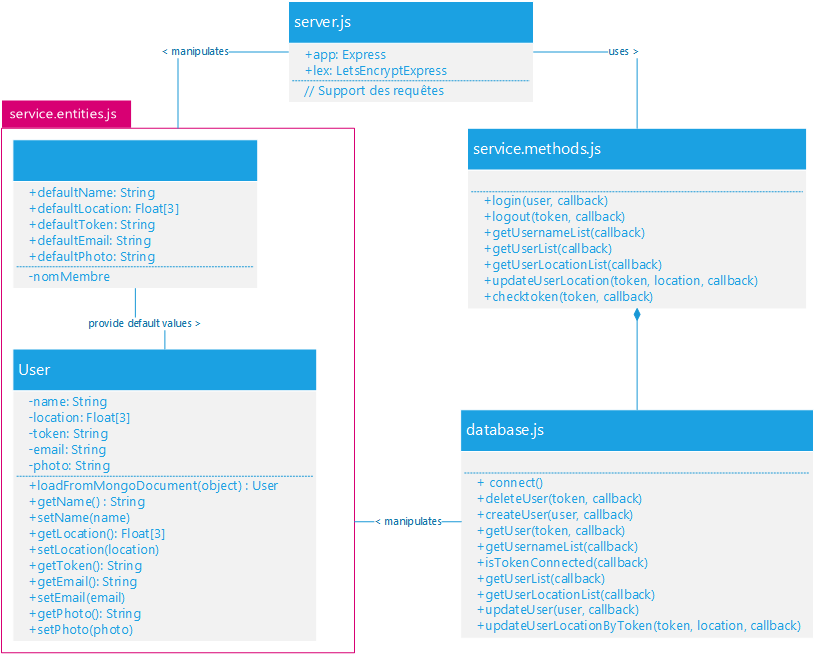
\includegraphics[width=\textwidth]{./img/architecture-service-web.png}
        \caption{Architecture du Service Web}
        \label{asweb}
    \end{figure}

    Comme nous pouvons l'observer dans la figure \ref{asweb}, nous distinguons plusieurs parties.

    La première partie concerne les entités que l'on va manipuler. Ces entités se trouvent dans un fichier \textbf{service.entities.js}. Nous allons retrouver une classe \textbf{User}, permettant de stocker et manipuler les utilisateurs connectés sur le service. Dans ce fichier se trouvent également des données par défaut à utiliser pour les utilisateurs qui ne renseigneraient pas leurs informations. Ceci permettra par la suite de disposer par exemple d'une photo à afficher par défaut pour un utilisateur qui ne la partage pas ou n'en a pas.

    Une autre partie importante va concerner le stockage des données. Ceci s'effectue par l'intermédiaire de la base de données. Avant de choisir une technologie, nous souhaitions qu'il soit possible de facilement modifier le gestionnaire de base de données (Oracle, MySQL, MongoDB, Microsoft Access).
    
    Pour que ceci se fasse plus facilement, il a été décidé de mettre en place un patron de conception "bridge" (à quelques exceptions, puisque Javascript ne dispose pas du concept d'interfaces).

    Nous remarquons donc dans la figure \ref{asweb} que notre fichier \textbf{database.js} dispose de méthodes manipulant les entités du service pour un certain type de base de données. Ce fichier et ensuite inclus dans le fichier \textbf{service.methods.js}, ce qui va permettre de les utiliser. Dans l'application, ce seront finalement les méthodes du fichier \textbf{service.methods.js} qui seront utilisées, permettant de masquer quel gestionnaire de base de données nous utilisons.
    
    Pour changer de gestionnaire de base de données, il suffit de créer un autre fichier, par exemple \textbf{database-sql.js}, d'y recréer les mêmes fonctions que dans le fichier \textbf{database.js} en modifiant la logique de celles-ci. Ensuite, il suffira simplement de modifier le fichier inclus dans \textbf{service.methods.js} par \textbf{database-sql.js}.

